\section*{Project plan}
\label{sec:project_plan}

\begin{figure}
  \centering
  \subbottom[]{%
    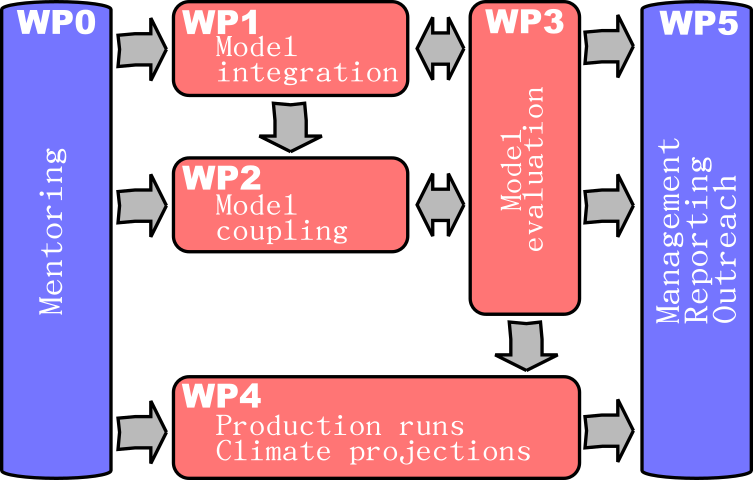
\includegraphics[width=0.48\linewidth]{wp_flow_chart}}
  \subbottom[]{%
    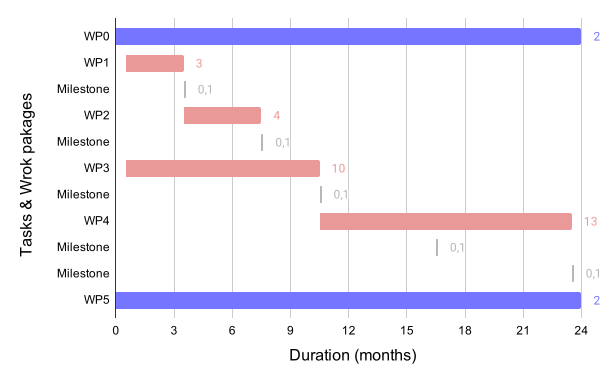
\includegraphics[width=0.48\linewidth]{chart}}
  \caption{Round}
\end{figure}

As specified in the call for the Lise-Meitner fellowship the project plan is aligned for a duration of 24 months. The project is divided into 5 \gls{wp} (Fig.~\ref{fig:flowchart}) of varying duration. \gls{wp}0 (Mentoring) and \gls{wp}5 (Management, reporting, and outreach) are designed to run through the whole project duration of 24 months concomitantly (Fig.~\ref{fig:ganttchart}). \gls{wp}0 incorporates support from the host institute. All outreach activity, including written and oral communication  is bundled in \gls{wp}5. The substantial work is assigned to \gls{wp}1-4. Technicality of the work packages is decreasing from \gls{wp}1 (purely technical) - \gls{wp}4 (purely scientific) with expected increasingly scientific throughput. \gls{wp}1 (Model integration) and \gls{wp}2 (Model coupling) are tightly interlinked with \gls{wp}3 (Model evaluation) spanning the whole duration of \gls{wp}1 and \gls{wp}2. \gls{wp}2 depends on the full-fillment \gls{wp}1. As does \gls{wp}4 depends on the full-fillment of all previous substantial work packages (1-3). The required full-fillment is marked with Milestones in Fig.~\ref{fig:ganttchart}. Milestones 3 and 4 also include reporting (deliverables?) to the funding agency.
 
\subsection*{\gls{wp}0 Mentoring}
\label{ssec:wp0}
The mentoring \gls{wp}, as described above spans the entire project periode and includes a variety of tasks in cooperation and with support of the host institute at BOKU. It is built upon the very core attributes of the Lise-Meitner fellowship call and shall grant a foundation for a sustainable position as a leader in my field of research. In the start phase of the project, I expect \gls{wp}0 to tend to friction free and efficient picking up of pace, both related to work environment and technical support at BOKU and scientific as well as social life in Austria in general. The mid-phase is dedicated to development and honing of key hard and soft skills necessary for a future leadership in science, including didactic and presentation techniques for public outreach. In the end-phase \gls{wp}0 will initiate the preparation of follow-up fellowship xx or stand-alone projects.\\

T0.1 Getting started and up to speed with institute and settle down in the country
T0.2 Setting up \gls{cesm} on institute/national infrastructure (info HR, HPC und support M.Alexander)
T0.3 Networking
T0.4 Personal skill development, project management and leadership
T0.5 Science didactic and presentation skills for public outreach
T0.6 Preparation of xx fellowship or regular project 

\subsection*{\gls{wp}1 Model integration}
\label{ssec:wp1}
The model integration \gls{wp} will incorporate and build on existing collaborations with technical and scientific stuff both at the University of Oslo (Norway) and at NCAR in Boulder (COL, US). Existing parts of the \gls{odina} model shall be extended to describe our current state of the art as best as possible. Which means including a state of stomata sluggishness to the \gls{odina} model and deduce additional parameters based on existing meta databases. In any case, it is expected that the model answer with active ozone damage will change from the reference simulation. Initial Cross-evaluation with data at global scales (coarse resolution model integration) following the CESM standard procedures are likely to reveal a necessity for fine tuning of free model parameters. In depth evaluation is subject to \gls{wp}3. In concert with \gls{wp}5 the \gls{wp}1 aimes to publish the \gls{odina} model as a model development paper as part of the indicated Milestone in Fig.~\ref{fig:ganttchart}.\\

T1.1 Extend \gls{odina} for sluggishness  
T1.2 Evaluate and adapt the integration of \gls{odina} in \gls{clm}~5 ($\rightarrow$ \gls{wp}3)
T1.3 Publish a development and evaluation paper on \gls{odina} ($\rightarrow$ \gls{wp}5)

\subsection*{\gls{wp}2 Model coupling}
\label{ssec:wp2}
The model coupling \gls{wp} will include a three month research stay at \gls{ncar}lab in Boulder, USA to both facilitate the technical work as well as build important networks for future work. Coupling to \gls{cam}-chem takes place in physical terms through the dry deposition implementation in CESM. The associated “reverse engineering task” will include in depth understanding and if necessary improvement and update of the existing dry deposition scheme within the framework of CESM. Technically this \gls{wp} involves touching the current model coupler infrastructure. At present it is known that the coupler infrastructure is subject to revision by the \gls{ncar} technical stuff. The coupling will be done in a sustainable way if possible within the new infrastructure. Results of the first coupled runs will be validated in coordination with \gls{wp}5 and in similar ways as described in \gls{wp}1.\\

T2.1 Reverse engineering of the dry deposition scheme and update if necessary 
T2.2 Technically coupling \gls{cam}-chem ozone concentrations to \gls{odina}
T2.3 Validation of model integrations

\subsection*{\gls{wp}3 Model evaluation and update of model parameters}
\label{ssec:wp3}
The model evaluation is an integral part of \gls{wp}1 and \gls{wp}2 and spans the whole duration of both. Initial integration and validation tests are complemented and completed with more in depth evaluation for selected sites (FluxNet) with associated ground level ozone observations which will be also collected in the course of \gls{wp}3. As mentioned in \gls{wp}1 and \gls{wp}2, it is foreseen that model parameters have to be adapted with respect to the reference simulation without ozone induced damage on photosynthesis and stomatal conductance. \gls{wp}4 aims towards a model evaluation paper in coordination with \gls{wp}5. The model development and evaluation paper could be synthesized into one if necessary.\\

T3.1 Collection of evaluation data 
T3.2 Site level evaluation (ideally relevant fluxnet sites with observed ozone)
T3.3 Global scale evaluation - surface ozone products (difficult - \gls{ecmwf} \gls{cam} reanalysis sucks) and GPP products (Sentinel satellites? there are issues with \gls{modis} here)
T 3.4 Update model parameters 
name in text: (e.g. $\mathrm{J_{max}}$0 in \gls{luna}, \glspl{pft}) and included “healing” methods
T3.4 Write evaluation paper

\subsection*{\gls{wp}4 Production runs and climate projections}
\label{ssec:wp4}
The work package for production runs with climate projections built upon the successful implementation of \gls{wp}1-3. It facilitates all previous work and will at least compare existing CMIP6 reference simulations of CESM for a selected high emission (low mitigation) scenario (\gls{ssp}5). The aim is to study the coupled effect of climate and ozone feedback on vegetation with respect for implications on future surface ozone abundance and hence air quality. A probable focus lies on Europe or other highly industrialized regions in East Asia.\\
 
T4.1 Run \gls{cesm} coupled of climatological timescales (at least one \gls{ssp})
T4.2 Study climate impact on surface ozone abundance 
name in text: along with plant damage, gpp

\subsection*{\gls{wp}5 Management, Reporting, Outreach}
\label{ssec:wp5}
As communication is an integral part of science the management \gls{wp} synergizes classical management like reporting to the funding agency with science communication and networking activities (conferences, workshopes). Science communication in \gls{wp}5 is regarded as separated into classical publications in the form of papers and public outreach. Latter might come in the form of popular science blogs or presentations to the general public. \gls{wp}5 spans the whole project duration and is the effective reporting hub for \gls{wp}1-4.\\
 
T5.1 Science communication
T5.1a Research papers
T5.1b Public outreach
T5.2 Networking: Conferences, Workshops
T5.3 Project reporting
